\documentclass{scrartcl}
\usepackage{graphicx}
\usepackage{amsmath}
\usepackage{listings}
\usepackage{mathtools}
\usepackage{physics}
\usepackage{siunitx}
\usepackage{tikz}
\usepackage{mathtools}
\usepackage{rotating}
\usepackage{hyperref}
\usepackage{fancyhdr}
\usepackage{float}

\pagestyle{fancy}
\fancyhf{}
\rhead{Jamie Grieser}
\lhead{Simulation Methods}
\rfoot{Page \thepage}

\definecolor{mygreen}{rgb}{0,0.6,0}
\definecolor{mygray}{rgb}{0.5,0.5,0.5}
\definecolor{mymauve}{rgb}{0.58,0,0.82}

\lstset{ 
	backgroundcolor=\color{white},   % choose the background color; you must add \usepackage{color} or \usepackage{xcolor}; should come as last argument
	basicstyle=\footnotesize,        % the size of the fonts that are used for the code
	breakatwhitespace=false,         % sets if automatic breaks should only happen at whitespace
	breaklines=true,                 % sets automatic line breaking
	captionpos=b,                    % sets the caption-position to bottom
	commentstyle=\color{mygreen},    % comment style
	deletekeywords={...},            % if you want to delete keywords from the given language
	escapeinside={\%*}{*)},          % if you want to add LaTeX within your code
	extendedchars=true,              % lets you use non-ASCII characters; for 8-bits encodings only, does not work with UTF-8
	frame=single,	                   % adds a frame around the code
	keepspaces=false,                 % keeps spaces in text, useful for keeping indentation of code (possibly needs columns=flexible)
	keywordstyle=\color{blue},       % keyword style
	language=Octave,                 % the language of the code
	morekeywords={*,...},            % if you want to add more keywords to the set
	numbers=left,                    % where to put the line-numbers; possible values are (none, left, right)
	numbersep=5pt,                   % how far the line-numbers are from the code
	numberstyle=\tiny\color{mygray}, % the style that is used for the line-numbers
	rulecolor=\color{black},         % if not set, the frame-color may be changed on line-breaks within not-black text (e.g. comments (green here))
	%showspaces=false,                % show spaces everywhere adding particular underscores; it overrides 'showstringspaces'
	showstringspaces=false,          % underline spaces within strings only
	showtabs=false,                  % show tabs within strings adding particular underscores
	stepnumber=2,                    % the step between two line-numbers. If it's 1, each line will be numbered
	stringstyle=\color{mymauve},     % string literal style
	tabsize=2,	                   % sets default tabsize to 2 spaces
	%title=\lstname                   % show the filename of files included with \lstinputlisting; also try caption instead of title
}

\begin{document}

\section*{Problem Sheet 10}
\subsection*{Exercise 1.1}
We want to solve the Riemann problem given on the sheet using two solvers, the classical and HLL-Riemann solver.
To do this, we us the following functions to run those algorithms which have been provided online.
\begin{lstlisting}[title=Function to initialize the initial conditions. We have to add one ghost cell at each boundary to make the algorithm work.,  language=Python, frame=single]
# Function to initialize the initial conditions
def initialize_initial_conditions(N):
	rho = np.zeros((N + 2))
	p = np.zeros((N + 2))
	u = np.zeros((N + 2))
	
	rho[0:int(np.floor(N/2))] = 1e5
	rho[int(np.floor(N/2)):] = 1.24e4
	
	p[0:int(np.floor(N / 2))] = 1
	p[int(np.floor(N / 2)):] = 0.1
	
	return rho, u, p
\end{lstlisting}
The following function was used to run the classical hydrodynamics solver in the adiabatic case.
After each iteration step, the \textit{calculate\_dt()} function is used to calulate the next time step such that the \textit{CFL-condition} is always satisfied properly.
The time step are summed up and the loop ends when it reaches the target time, which in our case is \( t = 5000 \).
Then it prints the result.
\begin{lstlisting}[title=Function to run the classical algorithm.,  language=Python, frame=single]
# Function to run the classical solver
def run_classical_solver(rho, u, p, time, N):
	q = np.zeros((3, N+2))
	q[0, :] = rho
	q[1, :] = u
	q[2, :] = p
	dt = 0.1
	t = 0
	while t < time:
		q = hydro_adi_classic_one_timestep(q, dx, dt)
		dt = calculate_dt(q)
		t += dt
		print('Time:', t)
	
	plot_results(q, N)
\end{lstlisting}
\newpage
We have exactly the same code for the HLL-Riemann solver, again with the variable timestep.
\begin{lstlisting}[title=Function to run the HLL-Riemann algorithm.,  language=Python, frame=single]
# Function to run the classical solver
def run_classical_solver(rho, u, p, time, N):
	q = np.zeros((3, N+2))
	q[0, :] = rho
	q[1, :] = u
	q[2, :] = p
	dt = 0.1
	t = 0
	while t < time:
		q = hydro_adi_riemann_one_timestep(q, dx, dt)
		dt = calculate_dt(q)
		t += dt
		print('Time:', t)
	
	plot_results(q, N)
\end{lstlisting}
The custom timesteps are calculated using the following function from \textit{sheet 9}.
\begin{lstlisting}[title=Function to run the HLL-Riemann algorithm.,  language=Python, frame=single]
# Recalculate dt at every step so that CFL is always satisfied
def calculate_dt(q):
	if np.amax(np.abs(q[1, :])) != 0:
		cfl = dx / (np.amax(np.abs(q[1, :])))
		dt = 0.4 * cfl
	else:
		dt = 0.1
	return dt
\end{lstlisting}
Figures \ref{fig:adiabatic200} and \ref{fig:adiabatic2000} display the results for both algorithms in the case of 200 and 2000 grid points respectively.
If we compare the 200 grid point case with the 2000 grid point case, we see that the flow features, that is the discontinuities are much sharper.
We also see that in both cases the classical solver predicts that the leftmost and rightmost boundaries travel a bit farther in the given time, resulting for example in the fact that the non-zero part of the velocity field is broader. 
It also predicts a much higher maximum speed.\\\\
In both figures, we see that both graphs have three regions where all fluid properties change, which are connected through sudden drops in the respective quantities.
From our intuition, we can easily identify the shock and rarefication waves as well as some kind of contact discontinuity.\\
As the density in the left half space is much higher, we expect a shock wave traveling from the left to the right and a rarefication wave traveling to the left.
The rightmost drop increases the initially low density in the right region suddenly to a much larger value and is thus the shock wave. Density, pressure and velocity are discontinuous there.
The classical algorithm also predicts that the shock wave is followed by a small rarefication wave, which is seen as a small dip before the density drop.
HLL-Riemann does not predict such a behavior, although it often happens in real scenarios.
On the other side we have the leftmost drop, where the density drops very fast from an initially very high value to a much lower value. 
It is not as dramatic as in the case of the shock, but still very string. This is the rarefication wave.
All the shown fluid properties are discontinuous there too.\\
Only the drop in the middle now remains to e explained. 
One is tempted to interpret it as a contact discontinuity, because it is sandwiched by a shock and a rarefication wave.
Also the pressure is almost equal on both sides when compared to the absolute value, as it is required by a contact discontinuity.
However, the velocity in both sides is certainly not zero and thus it is not a contact discontinuity, at least if one follows the definition of \textit{Landau-Lifshitz}.
Still, we interpret it like that. 
Both algorithms predict that it moves slightly to the right. \\\\

In the calculation above, we use Dirichlet boundary conditions and chose the boundaries to equal the initial conditions. 
From the simulation, we can deduce that the information (rarefication and shock waves) has not traveled far enough yet for boundary conditions to become important and thus the choice of our boundary conditions can be almost arbitrary.
For example, we could have chosen periodic boundary conditions which should then yield the same result.

\newpage

\begin{figure}[H]
	\centering
	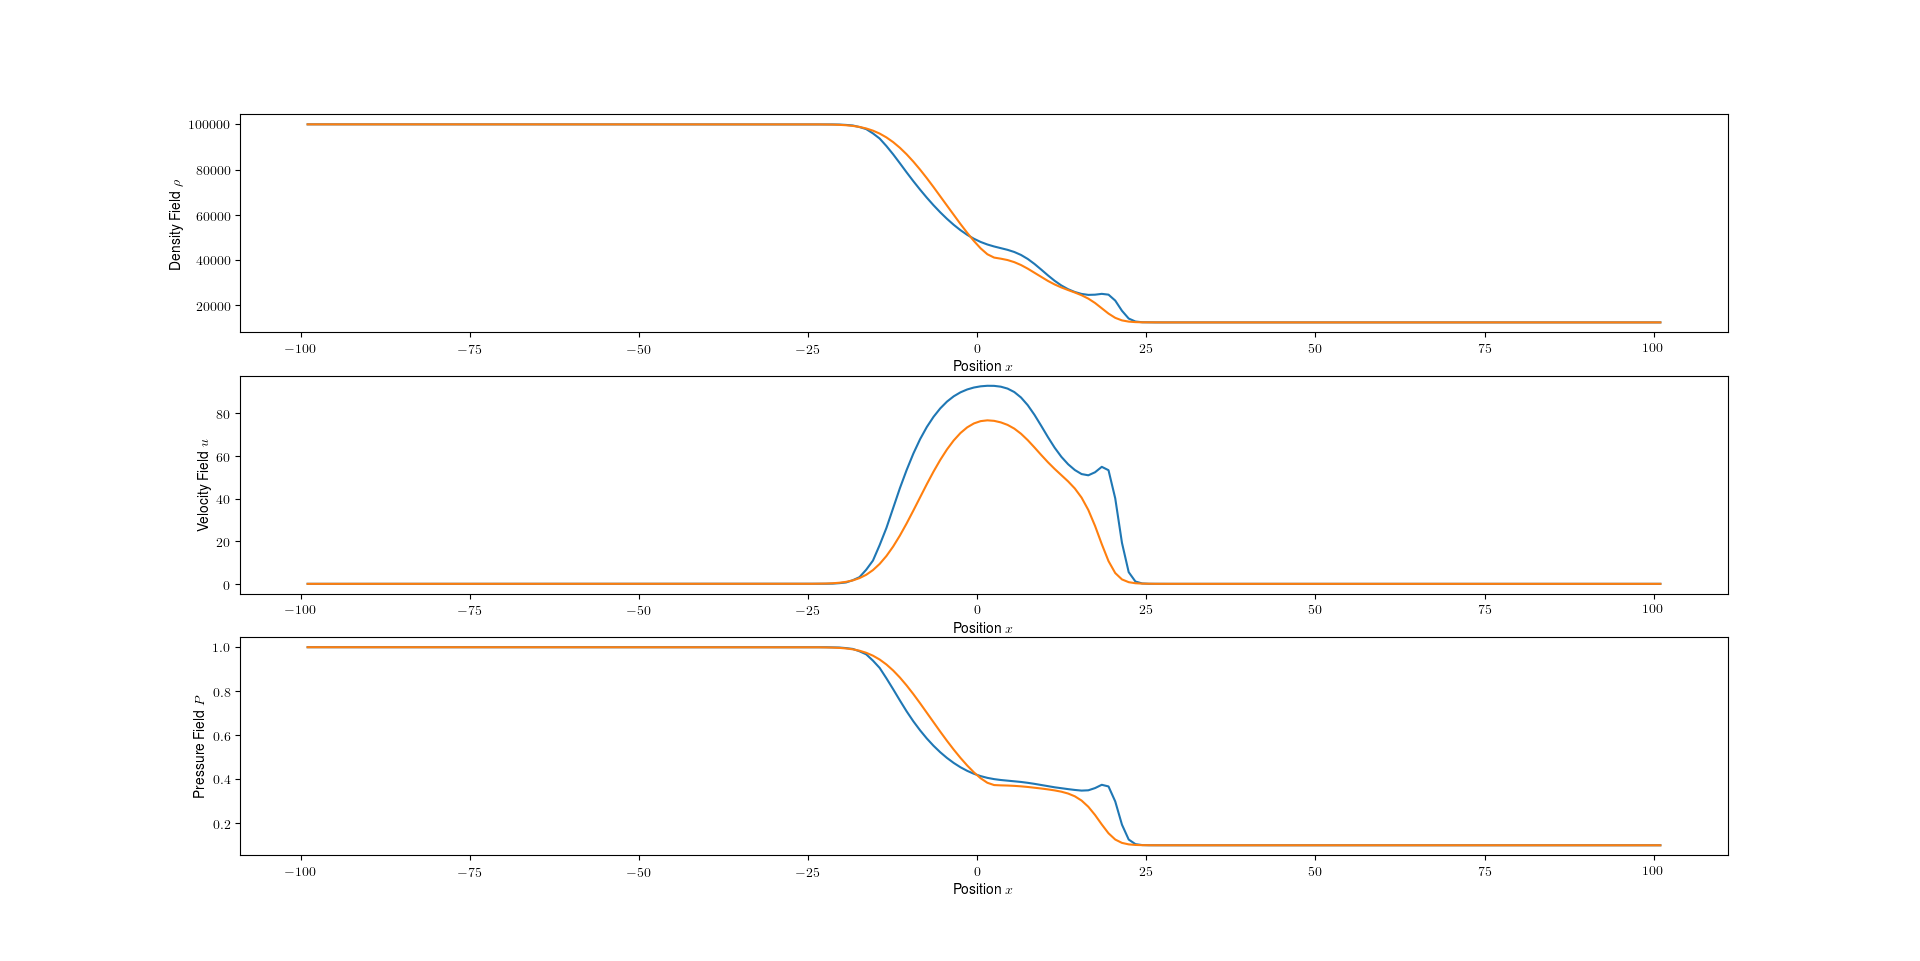
\includegraphics[width=1.0\linewidth]{../Adiabatic200}
	\caption{Density, velocity and pressure fields for 200 grid points. The blue graphs depict the classical solution, while the orange graph depicts the HLL-Riemann solution. }
	\label{fig:adiabatic200}
\end{figure}

\begin{figure}[H]
	\centering
	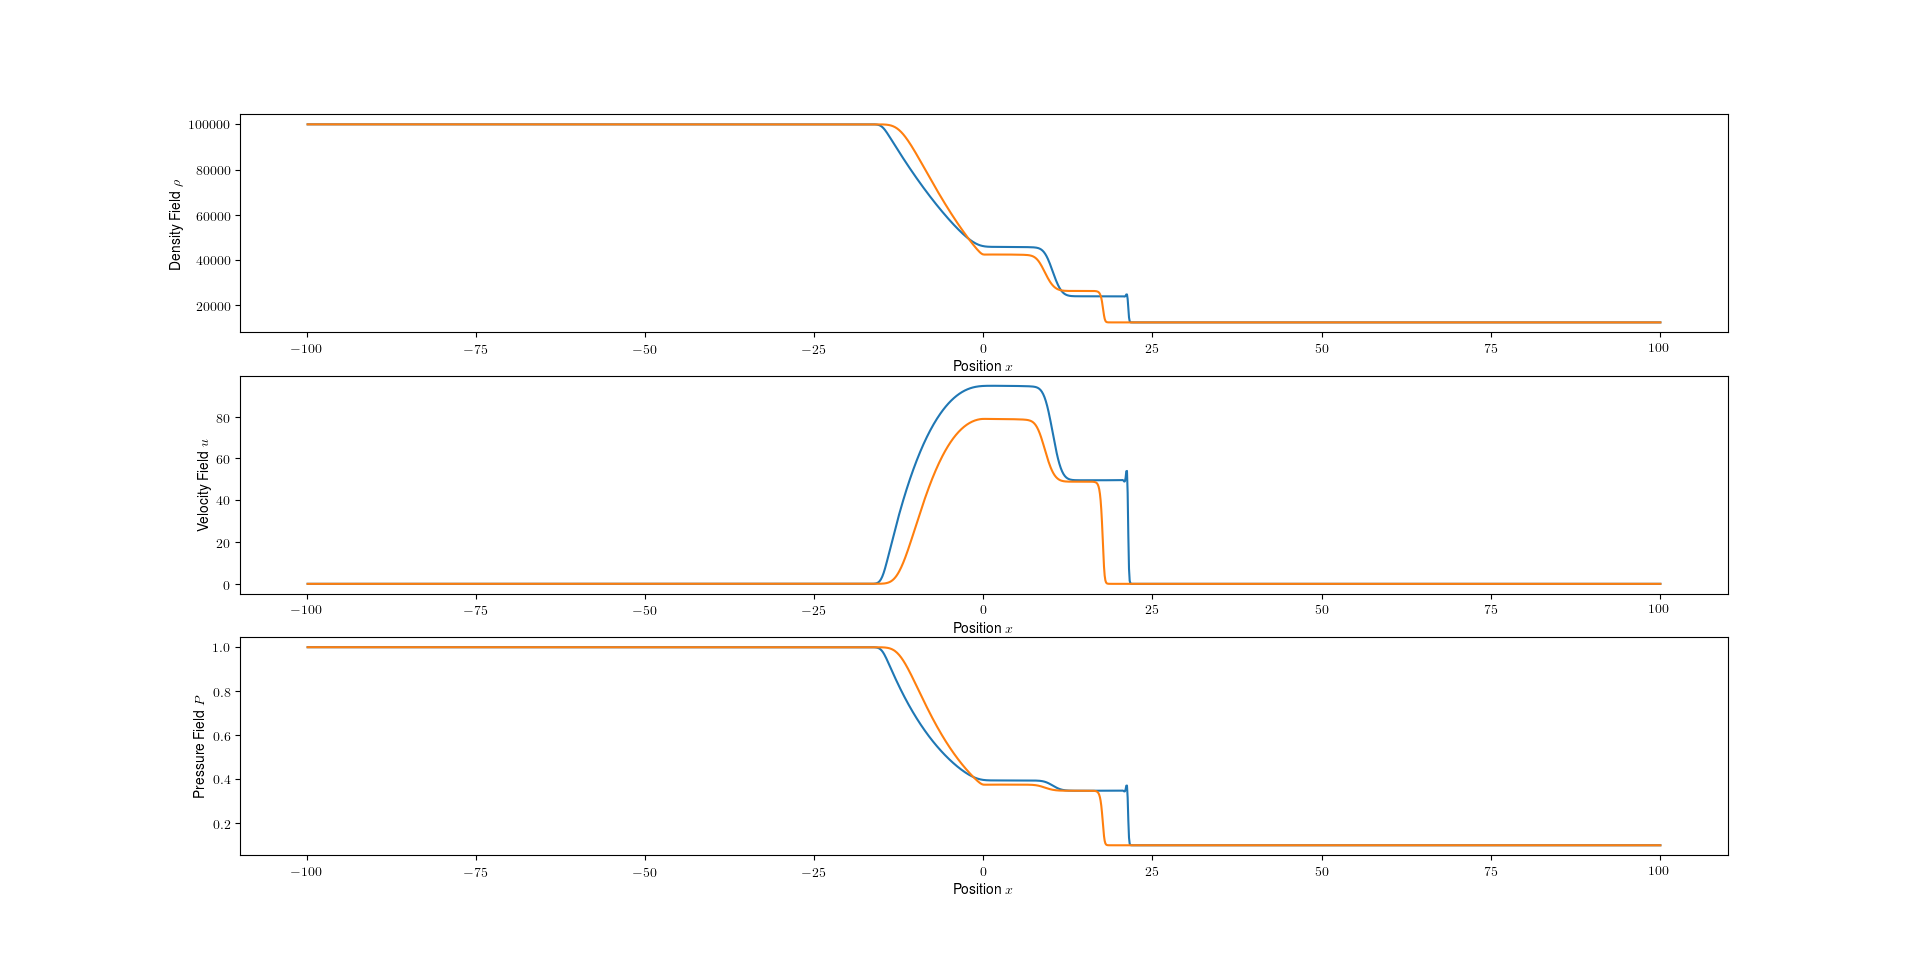
\includegraphics[width=1.0\linewidth]{../Adiabatic2000}
	\caption{Density, velocity and pressure fields for 2000 grid points. We see that the flow features are much sharper in comparison to the 200 grid point case.}
	\label{fig:adiabatic2000}
\end{figure}


\subsection*{Exercise 1.2}

We analyze a Kelvin-Helmholtz instability at the interface of two homogeneous fluid phases using the the \textit{Athena} MHD code.
The initial conditions have been implemented in the following way:

\begin{lstlisting}[title=Changes on the problem generator to implement the given initial conditions. A new variable du was introduced to implement the additional velocity term needed for exercise (c).,  language=C, frame=single]
/*** HERE CALCULATE YOUR DATA FOR THE MESH CELL (x1, x2, x3) ACCORDING TO THE PROBLEM AT HAND*/
double dens = 0 ;
double vx =   0 ;
double vy =   0 ;

double sigma = 0.01;
double du = 0.0;  // set to 5.0 to make computations for exercise (c)

dens = dens1 + (dens2 - dens1) / (1 + exp((x2 - 0.5) / sigma));
vx =   v1 + (v2 - v1) / (1 + exp((x2 - 0.5) / sigma)) + du;
vy = ampl * cos(kwave * x1) * exp(-kwave * abs(x2 - 0.5)) + du;

/************************************************************/
\end{lstlisting}

The parameter file was used to make computations for different resolutions starting from \( 64 \times 64 \) cells and then doubling the size until \( 512 \times 512 \) cells. 
We adjusted the resolution to \( 512 \times 512 \) pixels for every image for better comparison.
One can immediately see that the flow features get much cleaner for higher resolutions. 
If for example, we compare figure \ref{fig:kelvin64resize} with figure \ref{fig:kelvin512}, we see that in the \( 512 \times 512 \) the billows of the main waves even have smaller billows on them.
Those features are not even displayed in the low-resolution case.

\begin{figure}[H]
	\centering
	
\includegraphics[width=0.6\linewidth]{../Kelvin64_resize}
	\caption{Simulation of the Kelvin-Helmholtz instability on a \( 64 \times 64 \) grid.}
	\label{fig:kelvin64resize}
\end{figure}

\begin{figure}[H]
	\centering
	
\includegraphics[width=0.6\linewidth]{../Kelvin128_resize}
	\caption{Simulation of the Kelvin-Helmholtz instability on a \( 128 \times 128 \) grid.}
	\label{fig:kelvin128resize}
\end{figure}

\begin{figure}[H]
	\centering
	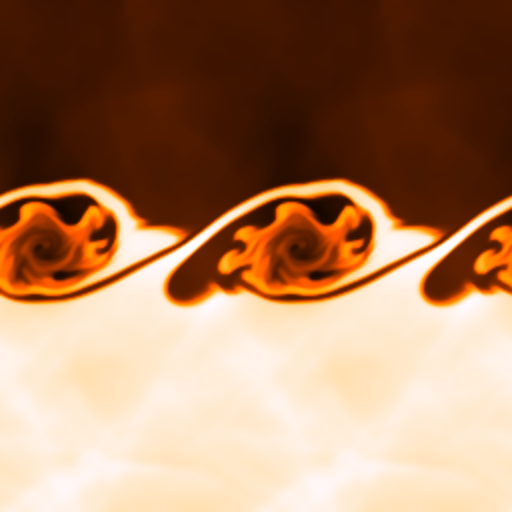
\includegraphics[width=0.6\linewidth]{../Kelvin256_resize}
	\caption{Simulation of the Kelvin-Helmholtz instability on a \( 256 \times 256 \) grid.}
	\label{fig:kelvin256resize}
\end{figure}

\begin{figure}[H]
	\centering
	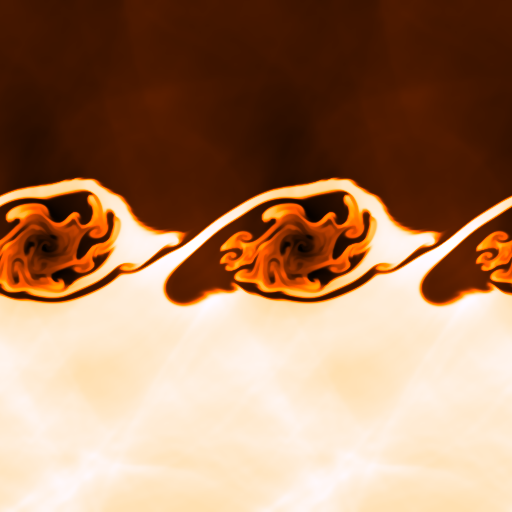
\includegraphics[width=0.6\linewidth]{../Kelvin512}
	\caption{Simulation of the Kelvin-Helmholtz instability on a \( 512 \times 512 \) grid.}
	\label{fig:kelvin512}
\end{figure}

To verify the linear growth rate, we can compare the logarithmic growth of the mean energy density in y-direction to the growth rate of the mode, which is given through
\begin{equation}\label{eq:growth}
	k \abs{u_1 - u_2}\frac{\sqrt{\rho_1\rho_2}}{\rho_1 + \rho_2} \cdot t
\end{equation}
where the constants \( k \), \( \rho_i \) and \( u_i \) are taken as given from the initial conditions.
The plots of these two quantities are shown in figure \ref{fig:growth}.\\
One sees that the growth rates are only approximately equal in the middle of the simulation for \( \SI{0.75}{\second}< t < \SI{1.5}{\second}\)
The reason for the growth rate being slower at the beginning is the face that we have a sharp boundary and only imprinted a slight perturbation with a small amplitude.
In the beginning, the change of energy density (and other fluid properties) in the interface region will therefore be very small, because without the density perturbation, we would have a stable system. \\
We also see that for \( t > \SI{2}{\second} \), the growth begins to stall.
This can be understood when we look at shape of the density field at late times.
We see that there, the fluid begins to mix within the billows and the differences in velocity and density are not as sharp anymore.
Thus, if we look at the growth rate \ref{eq:growth}, we see that it will decline, because it depends on the local difference in velocity as well as the the density.
The growth rate of the instabilities is much smaller.

\begin{figure}
	\centering
	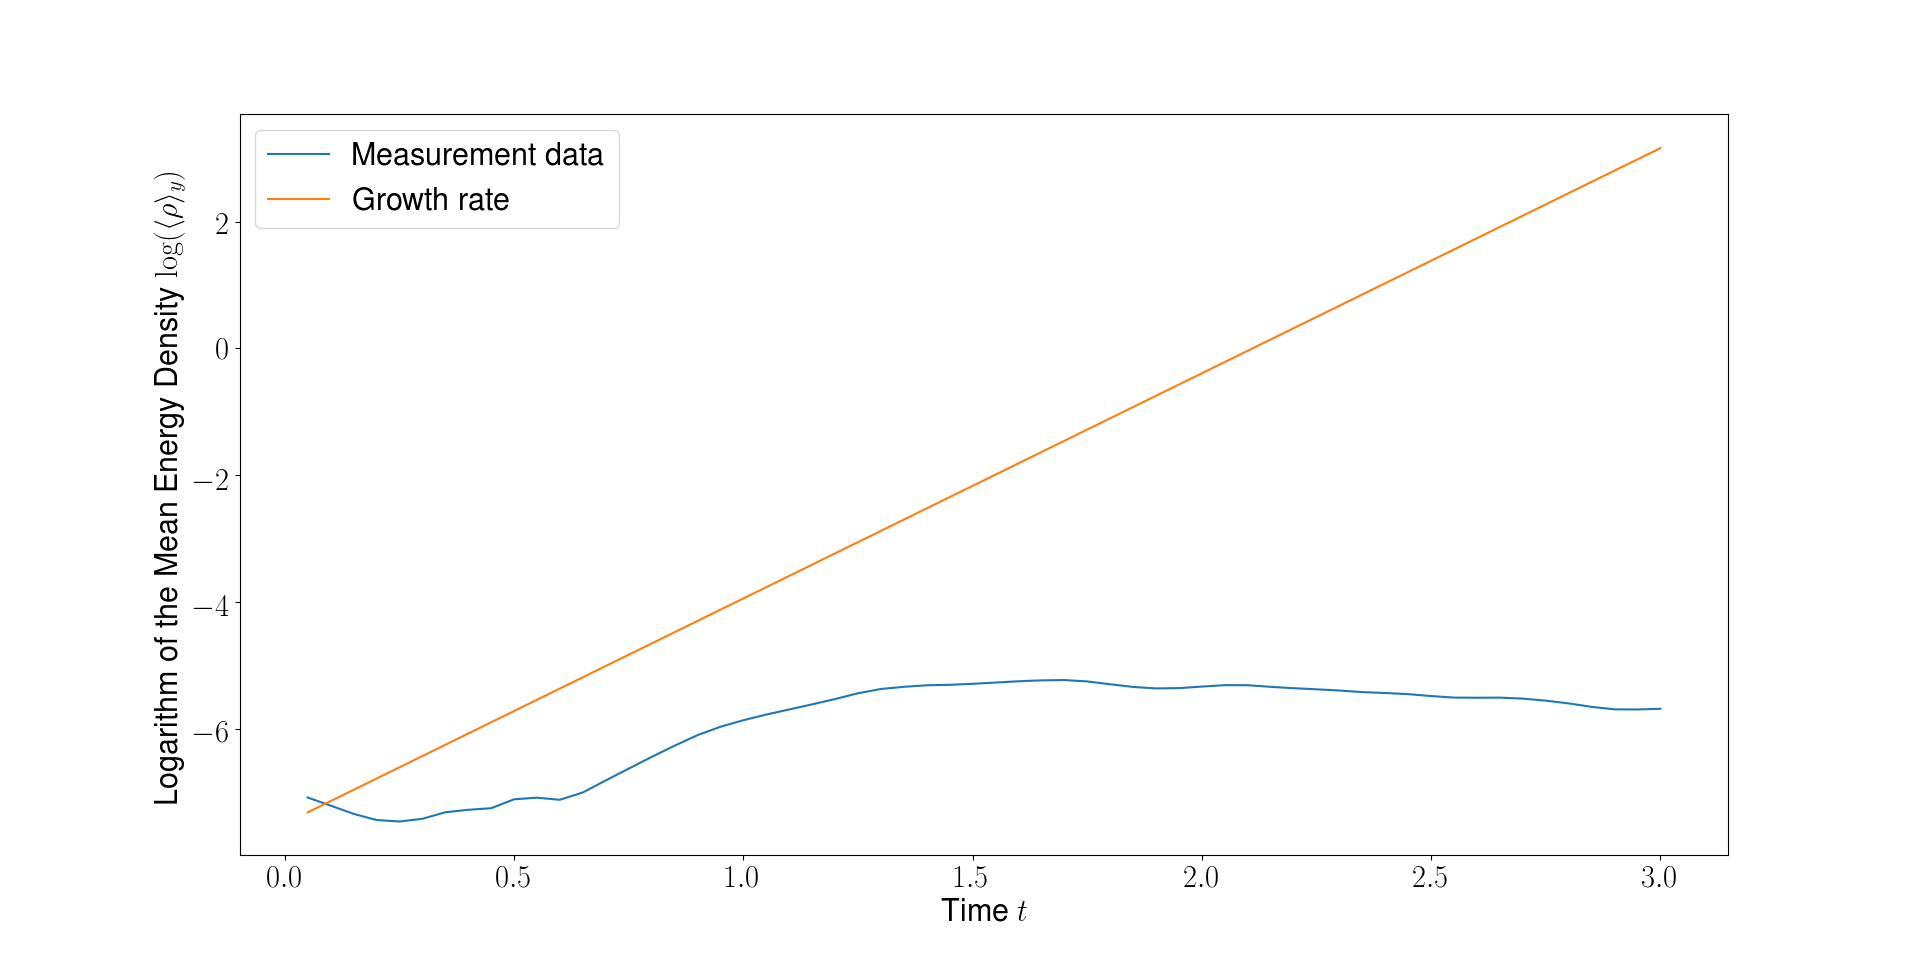
\includegraphics[width=0.9\linewidth]{../Growth}
	\caption{Growth of the mean energy density in y direction compared to the expected growth rate from theory.
	The expected growth rate was shifted, so that it offers better comparability.}
	\label{fig:growth}
\end{figure}

If we start adding a constant velocity to the initial condition in both directions (by setting \textit{du = 5.0}), we obtain the result displayed in figure \ref{fig:galileiinvarianceresize}.
It turns out that for large resolutions, the simulation begins to crash on our hardware and thus we did the simulation only on the \( 128 \times 128 \) grid.
The result looks quite different from what we would expect.
Our expectation would be that the shape of the instabilities is different from the \( \Delta u = 0.0 \)-case, but  the growth rate (compare equation \ref{eq:growth}) should be the same as we shifted both, \( u_1 \) and \( u_2 \) by the same rate.
As we can see, this is certainly not the case, because almost the entire fluid is perturbed by some instabilities now.
We can understand the result if we look at the boundary conditions. 
Our boundary conditions or the upper and lower boundaries are set to be reflecting.
If the velocity in y-direction is small, this approximation is good, because the interface does not travel  upward or downward. 
On the other hand, if the velocity of the interface is large, it gets reflected by the boundaries which then strongly contradicts the assumption of an infinitely big square.
Also, the perturbations due to the interface travel through the whole domain, causing a lot of disturbances.

\begin{figure}
	\centering
	
\includegraphics[width=0.7\linewidth]{../Galilei_Invariance_resize}
	\caption{Simulation with the new initial conditions where \( \Delta u = 5.0 \) on a \( 128 \times 128 \) grid.}
	\label{fig:galileiinvarianceresize}
\end{figure}



\end{document}
